\documentclass[journal]{IEEEtran}
\usepackage{cite}
\usepackage{amsmath,amssymb,amsfonts}
\usepackage{algorithmic}
\usepackage{graphicx}
\usepackage{textcomp}
\usepackage{xcolor}
\usepackage{booktabs}
\usepackage{subcaption}
\usepackage{hyperref}
\usepackage{algorithm}

% --- Abbreviation Macros ---
\newcommand{\ie}{\textit{i.e.}}
\newcommand{\eg}{\textit{e.g.}}
\newcommand{\etal}{\textit{et al.}}
\newcommand{\sgpmg}{\text{SG-PMG}}
\newcommand{\pmgdg}{\text{PMGDG}}


\begin{document}

\title{Semantic-Guided Progressive Domain Generalization for Hyperspectral Image Classification}

\author{Author~1,~\IEEEmembership{Member,~IEEE,} and Author~2,~\IEEEmembership{Member,~IEEE}%
\thanks{The authors are with the Department of Computer Science and Engineering.}
}

\markboth{IEEE Transactions on Geoscience and Remote Sensing,~Vol.~XX, No.~X, June~2026}%
{Authors: Semantic-Guided Progressive Domain Generalization for Hyperspectral Image Classification}

\maketitle

\begin{abstract}
Hyperspectral image (HSI) classification often suffers from performance degradation under geographical domain shifts due to variations in atmospheric and sensing conditions. Although domain generalization (DG) aims to learn domain-invariant representations without target domain access, existing DG methods often rely primarily on visual representations and lack explicit semantic guidance for robust cross-domain representation learning. Furthermore, progressive generation models remain limited in capturing transferable semantic relationships across domains, which can lead to semantic drift during progressive band synthesis. To address these limitations, we propose the Semantic-Guided Progressive Domain Generalization framework. Our method integrates class-level descriptions into a Prompt Bank using a frozen Contrastive Language-Image Pretraining (CLIP) text encoder. At each stage of the progressive spectral downsampling cascade, a Semantic-Aware Progressive Generator employs a Lightweight Image Encoder and a Multi-Head Cross Attention layer to perform semantic fusion between spatial features and prompt embeddings. The intermediate spatial-spectral representations are modulated via 3D Adaptive Layer Normalization (AdaLN3d) conditioned on pooled semantic features. A sub-discriminator evaluates the progressive multi-stage outputs using classification and projection heads, optimized via a semantic alignment loss. We train the framework using a two-stage strategy: Stage 1 pre-trains the generators, and Stage 2 trains a semantically aligned classifier on source and synthesized target-domain patches using Sharpness-Aware Minimization (SAM). The proposed framework consistently outperforms existing domain generalization methods on multiple benchmark HSI datasets. By grounding progressive generation in vision-language semantics, our method improves cross-domain representation learning and enhances generalization for hyperspectral image classification.
\end{abstract}


\begin{IEEEkeywords}
Hyperspectral image classification, domain generalization, progressive generation, cross-attention, adaptive normalization, Sharpness-Aware Minimization (SAM), vision-language alignment.
\end{IEEEkeywords}
\section{Introduction}
\label{sec:intro}

\IEEEPARstart{H}{yperspectral} imaging (HSI) sensors acquire continuous and finely divided spectral bands across the electromagnetic spectrum, capturing rich spatial-spectral cubes that characterize the physical properties of the Earth's surface. Consequently, HSI classification has emerged as a cornerstone technology in remote sensing, enabling precise land-cover mapping, precision agriculture, environmental monitoring, mineral and resource exploration, and natural disaster assessment~\cite{he2017deep}. Over the past decade, the rapid advancement of deep learning architectures, particularly convolutional neural networks (CNNs) and spatial-spectral Transformers, has dramatically improved classification performance by extracting hierarchical features from these high-dimensional cubes. However, HSI classification remains highly challenging in practical scenarios. The extremely high dimensionality of HSI data, coupled with variations in solar illumination, atmospheric scattering, sensor calibration, and geographical topography, leads to significant variations in spectral signatures. This creates a severe spectral-spatial distribution discrepancy between images captured in different regions or at different times, known as domain shift, which severely degrades the generalization capability of conventional deep learning models when evaluated on out-of-distribution scenes.

To address the performance drop caused by domain shift, transfer learning techniques have been widely researched. Unsupervised domain adaptation (DA) methods aim to align the feature distributions of the source and target domains by minimizing statistical discrepancies or using adversarial training~\cite{ehsnet2023}. However, DA methods are fundamentally limited by the requirement of accessing target domain samples during the model training phase. In real-world remote sensing applications, target-scene data are often completely unavailable during training, making DA impractical for immediate deployment. To circumvent this constraint, domain generalization (DG) has emerged as a more realistic and robust alternative. Unlike DA, DG aims to learn domain-invariant representations using only source domain data, such that the trained model generalizes directly to unseen target domains without any retraining or target data access~\cite{wang2022domain}. Nevertheless, cross-scene HSI domain generalization is exceptionally difficult. The unique, continuous spectral signatures of remote sensing ground objects are highly sensitive to minor environmental variations, leading to complex, non-linear distribution shifts that are difficult to model using only visual annotations from a single source domain.

To overcome the limitations of single-source HSI domain generalization, several approaches have been developed. These can be broadly categorized into generator-based style randomization methods and generator-free vision-language alignment models. Generator-based approaches, such as progressive domain expansion and style randomization frameworks~\cite{li2022progressive}, focus on simulating diverse target-domain distributions by progressively generating intermediate spectral bands and applying style perturbations to source samples. While effective at broadening the visual distribution coverage, these methods rely solely on visual transformations and are prone to generating unrealistic out-of-distribution samples. On the other hand, recent generator-free visual-language models leverage the cross-modal alignment capabilities of pre-trained models like CLIP~\cite{radford2021learning} to align HSI image patches with class-level textual descriptions in a shared semantic space. While these models capture high-level cognitive context, directly adapting them to high-dimensional remote sensing images remains challenging. Standard visual-language models are designed for three-channel natural images and struggle to extract the continuous spatial-spectral signatures and intricate physical properties of multi-band HSI cubes.

These limitations highlight a significant research gap in current HSI domain generalization. First, conventional progressive generation methods rely exclusively on visual-only style variations, which lack explicit semantic guidance. Without semantic constraints, progressive band synthesis often suffers from semantic inconsistency during domain generation, where the structural identity and class-specific layout of the generated patches are distorted. Second, existing methods exhibit insufficient semantic alignment across domains, as they align visual representations without grounding them in domain-invariant language concepts. Finally, the progressive synthesis of HSI bands suffers from weak semantic conditioning, relying on predefined or purely statistics-based band selection schemes during progressive spectral synthesis rather than dynamically integrating multimodal context to preserve class identity. These issues motivate the need for a framework that grounds the progressive generation and classification process in text-driven vision-language semantics, ensuring that generated target-domain variants preserve structural layouts and semantic consistency.

To address these limitations, we propose a Semantic-Guided Progressive Domain Generalization framework for cross-scene HSI classification. The proposed framework integrates high-level semantic descriptions into the progressive spatial-spectral generation process, establishing a unified vision-language learning paradigm. By utilizing a progressive spectral cascade, the model generates domain-generalized target-style variations of HSI patches while explicitly grounding intermediate feature representations in class-specific textual embeddings. This cross-modal guidance enforces semantic consistency during spectral band synthesis, preventing structural distortions and style-induced semantic drift. Finally, we optimize the network using a joint cross-domain semantic alignment strategy, guiding the classifier to capture transferable representations that generalize directly to unseen target domains.

The proposed framework offers several advantages for robust HSI domain generalization. By grounding progressive generation in class semantic representations, the model prevents semantic drift and preserves class-specific structural layouts during cross-domain feature translation. The semantic fusion mechanism enables dynamic alignment between spatial HSI features and textual description embeddings. Additionally, the adaptive semantic conditioning module dynamically modulates the intermediate features of the generator backbone, guiding the network to synthesize realistic target-domain variations. Finally, the robust optimization strategy ensures that the classification boundaries converge to flat loss regions, which stabilizes the training process and enhances generalization on unseen target distributions.

The primary contributions of this work are summarized as follows:
\begin{enumerate}
    \item We propose a novel cross-modal domain generalization paradigm that incorporates text-driven semantic guidance into a progressive generation framework, establishing a robust link between spatial-spectral features and high-level class concepts to mitigate semantic drift under geographical distribution shifts.
    \item We design a semantic-aware progressive generation mechanism that incorporates cross-modal feature fusion and adaptive conditioning, dynamically modulating intermediate spatial-spectral representations to preserve structural layout consistency across domain shifts.
    \item We develop a robust joint optimization framework based on cross-domain semantic alignment and flat-minima searching, ensuring that the model converges to generalize effectively across unseen target distributions.
    \item Extensive experiments on three public HSI benchmark datasets validate the domain generalization capability of our approach, demonstrating the effectiveness and competitiveness of the proposed framework under diverse cross-scene settings.
\end{enumerate}

\section{Related Work}
\label{sec:related}

\subsection{Domain Generalization for Hyperspectral Image Classification}
Domain generalization (DG) for hyperspectral image (HSI) classification aims to train a model on one or more source domains such that it generalizes directly to unseen target domains without target data access during training~\cite{wang2022domain}. In remote sensing, geographical domain shifts—caused by variations in atmospheric conditions, sensor specifications, and lighting angles—severely degrade the performance of traditional classification models. To address this issue, research trends have focused on expanding the model's generalization boundaries through data augmentation, domain-invariant feature extraction, or progressive generation. Data augmentation and style randomization frameworks, such as SDENet~\cite{sdenet2022} and LLURNet~\cite{llurnet2023}, focus on simulating diverse target-domain distributions by perturbing visual and spectral statistics. While these methods successfully broaden the visual search space, random perturbations applied directly to feature maps may not explicitly preserve the semantic layout or class structural information. Alternatively, domain-invariant representation learning and adversarial methods, such as FDGNet~\cite{fdgnet2022} and S2AMSNet~\cite{s2amsnet2022}, utilize discrepancy metrics or adversarial classifiers to isolate domain-specific variations from target-invariant features. While effective at aligning global statistics, these adversarial constraints may introduce semantic inconsistencies in the localized spatial-spectral representations. Finally, progressive generation methods, such as PMGDG~\cite{li2022progressive}, decompose the target domain simulation into sequential band generation steps. Although progressive schemes make high-dimensional generation tractable, the style perturbations applied at intermediate stages can limit cross-domain semantic consistency. Consequently, existing DG methods primarily rely on visual feature learning and often lack explicit semantic guidance to stabilize representation mapping during cross-domain generation.

\subsection{Vision-Language Learning for Hyperspectral Image Classification}
Vision-language learning has emerged as a powerful paradigm for cross-modal representation learning, spearheaded by foundation models like CLIP~\cite{radford2021learning} and ALIGN. By aligning visual patches and textual descriptions in a shared latent space via contrastive objectives, these models capture rich, domain-agnostic semantic concepts. In remote sensing, researchers have adapted vision-language concepts to scene classification and target detection to leverage the zero-shot generalization capabilities of linguistic priors. Specifically for HSI domain generalization, models like EHSNet~\cite{ehsnet2023} and asymmetric contrastive bridging models like ACB~\cite{acb2023} utilize class-level text descriptions to align visual feature maps in a text-guided latent space, improving the robust classification of out-of-distribution ground objects. While these approaches demonstrate the value of cross-modal alignment, adapting natural-image vision-language models to HSI remains highly challenging. First, standard vision-language models are designed for three-channel RGB images and struggle to extract the continuous spatial-spectral signatures of multi-band HSI cubes. Second, designing effective, context-rich textual prompts remains complex, often relying on manual annotation. Most importantly, existing visual-language models do not dynamically utilize language features to guide spatial-spectral generation. These limitations leave a critical gap: existing methods struggle to adapt vision-language representations dynamically to guide spatial-spectral synthesis, leading to insufficient semantic conditioning during feature generation.

\subsection{Progressive Generation and Semantic Alignment}
Progressive generation strategies decompose the modeling of complex, high-dimensional target distributions into a cascade of lower-dimensional generation steps. For HSI domain generalization, progressive domain expansion and step-wise spectral downsampling cascades make the optimization of high-dimensional HSI patches tractable, simulating realistic target-domain variations. Existing progressive generation models primarily focus on expanding visual diversity and learning domain-invariant representations through feature generation. By partitioning the high-dimensional HSI bands into progressive spectral steps, these methods reduce the complexity of the feature translation task. Conversely, recent vision-language methods mainly focus on improving semantic representation learning through cross-modal image-text alignment in a shared latent space.

However, these two research directions are largely studied independently. Integrating semantic guidance throughout the progressive generation process to improve domain-invariant feature generation remains relatively underexplored in HSI domain generalization. Incorporating semantic guidance has the potential to preserve class semantics during the progressive generation steps, improving the semantic consistency and transferability of generated feature representations. To address these limitations, we present a unified framework in the next section that combines progressive generation, semantic guidance, vision-language alignment, and adaptive semantic conditioning.

\section{Methodology}
\label{sec:methodology}

\subsection{Overall Framework}
The proposed Semantic-Guided Progressive Domain Generalization framework is designed to learn robust, transferable representations for cross-scene HSI classification using only source-domain data. The overall framework is illustrated in Fig. 1. As shown in Fig. 1, the proposed framework consists of two training stages: Stage 1 performs progressive semantic domain generation to pre-train generators and discriminators, and Stage 2 performs semantically aligned classifier training using Sharpness-Aware Minimization (SAM). The target style generation is decomposed into hierarchical spectral downsampling steps to stabilize training. In Stage 1, a Semantic-Aware Progressive Generator processes downsampled spectral steps, dynamically fusing spatial textures from a Lightweight Image Encoder with class-specific text representations from a Prompt Bank via cross-attention and Adaptive Layer Normalization (AdaLN3d). Sub-discriminators evaluate these outputs using classification, projection, and semantic alignment heads. In Stage 2, the pre-trained generators are frozen to synthesize out-of-distribution variations, building an expanded training set to optimize a robust classifier under flat-minima constraints.

\begin{figure*}[t]
\centering
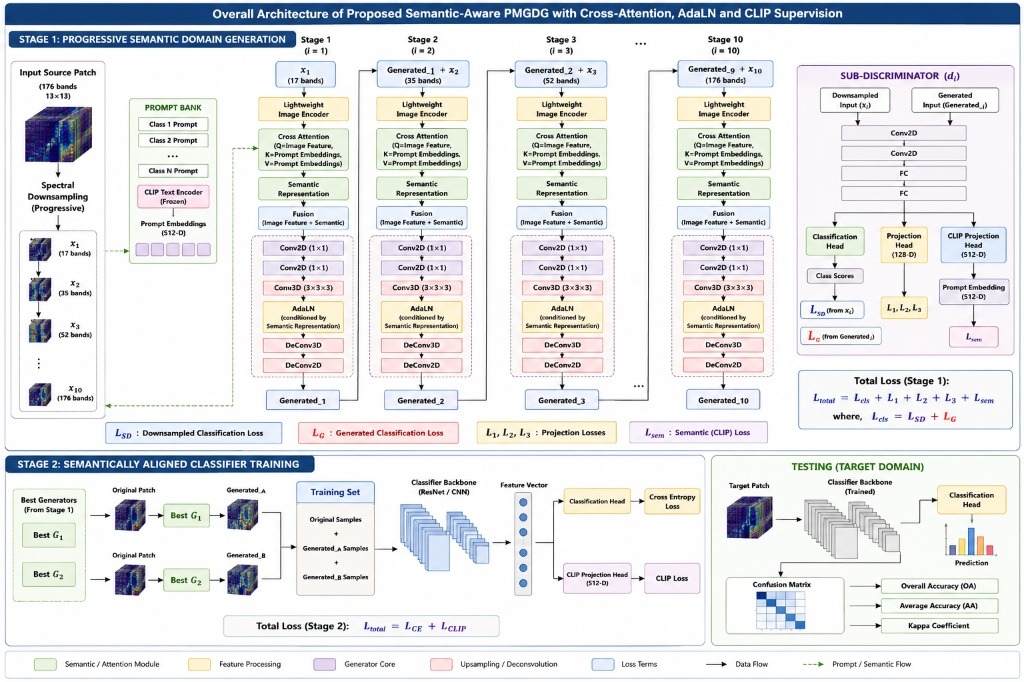
\includegraphics[width=0.95\textwidth]{architecture.jpg}
\caption{Detailed schematic flow of the proposed Semantic-Guided Progressive Domain Generalization framework. Stage 1 pre-trains progressive semantic-aware generators and discriminators on downsampled spectral steps. Stage 2 trains the final classifier on a joint set of original and generated patches using Sharpness-Aware Minimization (SAM) and cross-modal contrastive alignment.}
\label{fig:architecture}
\end{figure*}

\subsection{Problem Formulation}
To define the domain generalization task, we represent the spatial-spectral remote sensing datasets mathematically. Let the labeled source domain be denoted by $\mathcal{D}_S = \{(\mathbf{x}_i^s, y_i^s)\}_{i=1}^{N_S}$, where $N_S$ is the number of training samples, $\mathbf{x}_i^s \in \mathbb{R}^{H \times W \times C_s}$ represents the spatial-spectral HSI patch with spatial dimension $H \times W$ and spectral bands $C_s$, and $y_i^s \in \{1, 2, \dots, N_c\}$ is the class label among $N_c$ categories. Let the target domain be denoted by $\mathcal{D}_T = \{\mathbf{x}_j^t\}_{j=1}^{N_T}$. In our generalization setup, only source-domain data are used during training, and no target-domain information is accessed during optimization. The objective is to learn a mapping function $f: \mathbf{x} \to y$ that generalises to unseen target domain variations under domain shift:
\begin{equation}
\min_{f} \mathbb{E}_{\mathbf{x}^t, y^t \sim \mathcal{D}_T} \left[ \mathbb{I}(f(\mathbf{x}^t) \neq y^t) \right]
\end{equation}
where $\mathbb{I}(\cdot)$ is the indicator function, and $\mathbf{x}^t, y^t$ are samples from the unseen target distribution.

\subsection{Progressive Spectral Downsampling}
Due to the high dimensionality and spectral redundancy of HSIs, generating target-domain styles directly in a single step can lead to unstable training. To address this, we decompose the patch spectral bands into $K$ progressive stages. At each stage $k \in \{1, \dots, K\}$, the downsampling function $\Phi_k: \mathbb{R}^{H \times W \times C_s} \to \mathbb{R}^{H \times W \times C_k}$ averages adjacent spectral slices into $C_k$ groups, mapping the input patch $\mathbf{x}$ to a downsampled step $\mathbf{x}_k \in \mathbb{R}^{H \times W \times C_k}$:
\begin{equation}
\mathbf{x}_k(h, w, j) = \frac{1}{|S_j|} \sum_{c \in S_j} \mathbf{x}(h, w, c)
\end{equation}
where $S_j$ is the index set of the $j$-th spectral channel group, $|S_j|$ is the group size, and $C_1 < C_2 < \dots < C_K = C_s$.

\subsection{Semantic Guidance}
To guide style translation without altering the underlying category layout, we construct a Vision-Language Prompt Bank. The class category description $t_c$ is embedded using a frozen pre-trained CLIP text encoder $\mathbf{\Psi}_{text}$ into prompt embeddings $\mathbf{e}_c \in \mathbb{R}^{512}$:
\begin{equation}
\mathbf{e}_c = \mathbf{\Psi}_{text}(t_c)
\end{equation}
where $t_c$ represents the textual template corresponding to class $c$. To avoid redundant computation, these static embeddings are computed once and stored in the prompt matrix $\mathbf{E}_{txt} \in \mathbb{R}^{N_c \times 512}$.

\subsection{Semantic-Aware Progressive Generator}
At each stage $k$, the generator uses a visual-semantic pipeline to reconstruct the target HSI patch from the downsampled input $\mathbf{x}_k$.

\subsubsection{Multi-Head Cross Attention}
To associate spatial features with textual descriptions, query, key, and value representations are computed. The visual feature map $\mathbf{F}_{img} \in \mathbb{R}^{H \times W \times C_k}$ extracted from the lightweight encoder is flattened to sequence $\mathbf{F}_{flat} \in \mathbb{R}^{HW \times C_k}$ and projected to Queries, while class prompt embeddings $\mathbf{E}_{txt}$ are projected to Keys and Values:
\begin{equation}
\mathbf{Q} = \mathbf{F}_{flat} \mathbf{W}_Q, \quad \mathbf{K} = \mathbf{E}_{txt} \mathbf{W}_K, \quad \mathbf{V} = \mathbf{E}_{txt} \mathbf{W}_V
\end{equation}
where $\mathbf{W}_Q \in \mathbb{R}^{C_k \times d_{model}}$, $\mathbf{W}_K \in \mathbb{R}^{512 \times d_{model}}$, and $\mathbf{W}_V \in \mathbb{R}^{512 \times d_{model}}$ project features to dimension $d_{model} = 512$. Cross attention is formulated as:
\begin{equation}
\mathbf{F}_{attn} = \text{softmax}\left(\frac{\mathbf{Q} \mathbf{K}^T}{\sqrt{d_{model}}}\right) \mathbf{V} \mathbf{W}_O
\end{equation}
where $\mathbf{W}_O \in \mathbb{R}^{d_{model} \times C_k}$ is the output projection weight, and $\mathbf{F}_{attn} \in \mathbb{R}^{HW \times C_k}$ is the cross-attention output. Injecting semantic representations step-by-step prevents style-induced semantic drift.

\subsubsection{Semantic Fusion}
To combine visual textures and linguistic concepts dynamically, we use a gated fusion layer:
\begin{equation}
\mathbf{G} = \sigma\left(\left[\mathbf{F}_{flat} \parallel \mathbf{F}_{attn}\right] \mathbf{W}_{gate} + \mathbf{b}_{gate}\right)
\end{equation}
\begin{equation}
\mathbf{F}_{fusion} = \mathbf{F}_{img} + \alpha \cdot \text{Reshape}\left(\mathbf{G} \odot \mathbf{F}_{flat} + (\mathbf{1} - \mathbf{G}) \odot \mathbf{F}_{attn}\right)
\end{equation}
where $\mathbf{W}_{gate} \in \mathbb{R}^{2C_k \times C_k}$ and $\mathbf{b}_{gate} \in \mathbb{R}^{C_k}$ represent the gate weights and biases, $\sigma$ is the sigmoid function, $\alpha = 0.1$ is a learnable scaling parameter, and $\parallel$ is feature concatenation.

\subsubsection{Adaptive AdaLN}
To modulate intermediate HSI representation based on class semantics, we pool $\mathbf{F}_{sem}$ (the reshaped fused features) to semantic condition vector $\mathbf{v}_{sem} \in \mathbb{R}^{C_k}$ and project it to scaling $\mathbf{\gamma}$ and shifting $\mathbf{\beta}$ parameters:
\begin{equation}
\mathbf{\gamma}, \mathbf{\beta} = \text{Split}\left(\text{Linear}(\mathbf{v}_{sem})\right)
\end{equation}
The Adaptive Layer Normalization (AdaLN3d) operation on 3D intermediate backbone tensor $\mathbf{V}_{3D}$ is defined as:
\begin{equation}
\text{AdaLN3d}(\mathbf{V}_{3D}, \mathbf{v}_{sem}) = (\mathbf{1} + \mathbf{\gamma}) \odot \left(\frac{\mathbf{V}_{3D} - \mu(\mathbf{V}_{3D})}{\sqrt{\sigma^2(\mathbf{V}_{3D}) + \epsilon}}\right) + \mathbf{\beta}
\end{equation}
where $\mu$ and $\sigma^2$ denote the mean and variance computed over the channel dimension, and scale and shift are clamped to prevent gradient instability: $\mathbf{\gamma} = \text{clamp}(\mathbf{\gamma}, -0.9, 2.0)$ and $\mathbf{\beta} = \text{clamp}(\mathbf{\beta}, -3.0, 3.0)$.

\subsubsection{Progressive Reconstruction}
The fused spatial-spectral feature map is projected to PCA space via a $1 \times 1$ Conv2D, reshaped to a 3D volume, processed by Conv3D, normalized using AdaLN3d, upsampled with DeConv3D, and reconstructed to target spectral dimensions via a $1 \times 1$ Conv2D (DeConv2D):
\begin{equation}
\mathbf{x}_{gen} = \text{DeConv2D}\left(\text{DeConv3D}\left(\mathbf{V}_{norm}\right)\right)
\end{equation}
where $\mathbf{V}_{norm}$ is the AdaLN3d modulated feature map, and $\mathbf{x}_{gen} \in \mathbb{R}^{H \times W \times C_k}$ represents the generated target-style patch.

\subsection{Sub-Discriminator}
To evaluate the progressive multi-stage outputs, each stage $k$ utilizes a sub-discriminator $\mathbf{d}_k$ equipped with three heads: classification score head predicting class scores $\mathbf{p}_{cls}$, projection head mapping features to $\mathbf{z}_{proj} \in \mathbb{R}^{128}$, and CLIP projection head mapping features to $\mathbf{z}_{clip} \in \mathbb{R}^{512}$.

\subsection{Semantic Alignment}
To align the visual representations with prompt embeddings, we minimize a cross-modal contrastive classification loss over HSI patch CLIP projections and text prompt embeddings:
\begin{equation}
\mathcal{L}_{sem} = -\frac{1}{B} \sum_{i=1}^B \log \frac{\exp\left(\tau \cdot \mathbf{z}_{clip, i} \mathbf{e}_{y_i}^T\right)}{\sum_{j=1}^{N_c} \exp\left(\tau \cdot \mathbf{z}_{clip, i} \mathbf{e}_j^T\right)}
\end{equation}
where $\mathbf{z}_{clip, i}$ is the CLIP projection of the $i$-th HSI patch in a batch of size $B$, $\mathbf{e}_{y_i}$ is the prompt embedding of the ground-truth class, and $\tau$ is a temperature scaling parameter.

\subsection{Two-Stage Training}
\subsubsection{Stage 1: Generator Pre-training}
During Stage 1, we optimize the progressive generators and sub-discriminators. We define the general contrastive loss $\mathcal{L}_{con}$ for a batch $I$ with views $A(i)$ and class mates $P(i)$ as:
\begin{equation}
\mathcal{L}_{con}(\mathbf{Z}, y, adv) = \sum_{i \in I} \frac{-1}{|P(i)|} \sum_{p \in P(i)} \log \Psi(i, p, adv)
\end{equation}
where $\Psi(i, p, adv)$ represents the alignment probability:
\begin{equation}
\Psi(i, p, adv) = \begin{cases}
    \frac{\exp(\mathbf{z}_i \cdot \mathbf{z}_p / \tau)}{\sum_{a \in A(i)} \exp(\mathbf{z}_i \cdot \mathbf{z}_a / \tau)} & adv=\text{False} \\
    1 - \frac{\exp(\mathbf{z}_i \cdot \mathbf{z}_p / \tau)}{\sum_{a \in A(i)} \exp(\mathbf{z}_i \cdot \mathbf{z}_a / \tau)} & adv=\text{True}
\end{cases}
\end{equation}
The downsampled consistency loss $\mathcal{L}_{wd}$ aligns original features $\mathbf{z}_{whole}$ and PCA-downsampled features $\mathbf{z}_{down}$:
\begin{equation}
\mathcal{L}_{wd} = \mathcal{L}_{con}([\mathbf{z}_{whole} \parallel \mathbf{z}_{down}], y, \text{False})
\end{equation}
The total discriminator loss at stage $k$ is:
\begin{equation}
\mathcal{L}_{total}^D = \mathcal{L}_{SD} + \lambda_1 \mathcal{L}_{1} + \lambda_{sem} \mathcal{L}_{sem}^D
\end{equation}
where $\mathcal{L}_{SD} = \mathcal{L}_{CE}(\mathbf{p}_{down}, y) + \mathcal{L}_{CE}(\mathbf{p}_{gen}, y)$ evaluates class correctness, and $\mathcal{L}_1$ is the interclass projection contrastive loss computed using $\mathcal{L}_{con}$. The generator is trained using:
\begin{equation}
\mathcal{L}_{total}^G = \mathcal{L}_{G} + \lambda_2 \mathcal{L}_{2} + \lambda_{sem} \mathcal{L}_{sem}^G
\end{equation}
where $\mathcal{L}_2$ is the intraclass adversarial contrastive loss, and $\mathcal{L}_G = \mathcal{L}_{CE}(\mathbf{p}_{gen}, y)$.

\subsubsection{Stage 2: Classifier Training}
The pre-trained generators $G_1, G_2$ are frozen to construct a joint training set of original source patches and synthesized target variations:
\begin{equation}
\mathbf{X}_{train} = \left[\mathbf{x} \parallel G_1(\mathbf{x}) \parallel G_2(\mathbf{x})\right]
\end{equation}
The final classifier parameters $\theta$ are trained using SAM. SAM searches for parameters in flat loss regions:
\begin{equation}
\theta \leftarrow \theta - \eta \nabla_{\theta} \mathcal{L}_{Stage2}(\theta + \epsilon(\theta))
\end{equation}
where $\epsilon(\theta) = \arg\max_{\|\epsilon\| \le \rho} \mathcal{L}_{Stage2}(\theta + \epsilon)$, and $\rho$ is the perturbation radius. The Stage 2 joint loss is formulated as:
\begin{equation}
\mathcal{L}_{Stage2} = \mathcal{L}_{CE}(\mathbf{p}_{cls}, y_{total}) + \lambda_{clip} \mathcal{L}_{clip}
\end{equation}
where $\mathcal{L}_{clip}$ is the contrastive CLIP loss computed over the expanded batch of size $3B$:
\begin{equation}
\mathcal{L}_{clip} = -\frac{1}{3B} \sum_{i=1}^{3B} \log \frac{\exp\left(\tau \cdot \mathbf{z}_{clip, i} \mathbf{e}_{y_{total, i}}^T\right)}{\sum_{j=1}^{N_c} \exp\left(\tau \cdot \mathbf{z}_{clip, i} \mathbf{e}_j^T\right)}
\end{equation}

\subsection{Testing / Inference}
During testing, generators are discarded. Inference is performed directly on unseen target HSI patches $\mathbf{x}^t \in \mathcal{D}_T$ using the classifier backbone to calculate classification accuracy. No target-domain images are accessed during training. Evaluation is performed using Overall Accuracy (OA), Average Accuracy (AA), and the Kappa coefficient.

\subsection{Training Algorithm}
\label{sec:algorithm}

Algorithm~\ref{alg:training} summarizes the complete two-stage training procedure of the proposed SG-PMG framework.

\begin{algorithm}[H]
\caption{Two-Stage Training Procedure of SG-PMG}
\label{alg:training}
\begin{algorithmic}[1]
\REQUIRE Source dataset $\mathcal{D}_s = \{(\mathbf{x}_i, y_i)\}$, Target dataset $\mathcal{D}_t = \{\mathbf{x}_j^t\}$, target class prompt bank $\mathbf{E}_{txt}$, batch size $B$, stage epochs $E_1, E_2$, progressive steps $K$, scaling weights $\lambda_1, \lambda_2, \lambda_{sem}, \lambda_{clip}$.
\ENSURE Optimized classifier $D_{net}$.

\STATE Load CLIP model on device; compute cached text features $\mathbf{E}_{txt}$.
\STATE Initialize progressive networks $g_1, g_2, d_1, d_2$.

\STATE \COMMENT{\textbf{STAGE 1: Progressive Generator Pre-training}}
\FOR{epoch = 1 \TO $E_1 \cdot K$}
    \STATE Calculate current progressive step: $k = \lfloor \text{epoch}/E_1 \rfloor + 1$.
    \FOR{each mini-batch $(\mathbf{X}, \mathbf{y}) \in \mathcal{D}_s$}
        \STATE Extract class prompts: $\mathbf{e}_y = \text{Index}(\mathbf{E}_{txt}, \mathbf{y})$.
        \STATE $\mathbf{X}_g, \mathbf{X}_{down} \leftarrow \text{Forward}(g_1, \mathbf{X}, k, \mathbf{e}_y, \mathbf{E}_{txt})$.
        \STATE Compute downsampled consistency loss: $\mathcal{L}_{wd} \leftarrow \mathcal{L}_{con}([\mathbf{z}_{whole} \parallel \mathbf{z}_{down}], \mathbf{y})$.
        \STATE Compute discriminator loss $\mathcal{L}_{1\_1}$ using class and semantic losses.
        \STATE Compute generator style adversarial loss: $\mathcal{L}_{2\_1} \leftarrow \text{CE}(\mathbf{p}_{tgt}, \mathbf{y}) + \lambda_2 \mathcal{L}_{adv} + \lambda_{sem} \mathcal{L}_{sem}$.
        \STATE Update $d_1$ and $g_1$ parameters using Adam optimizers.
        \STATE Repeat updates for $d_2$ and $g_2$.
    \ENDFOR
\ENDFOR

\STATE \COMMENT{\textbf{STAGE 2: SAM-Guided Classifier Tuning}}
\STATE Initialize standalone classifier $D_{net}$; load weights from the final pre-trained sub-discriminator $d_1[-1]$.
\FOR{epoch = 1 \TO $E_2$}
    \FOR{each mini-batch $(\mathbf{X}, \mathbf{y}) \in \mathcal{D}_s$}
        \STATE $\mathbf{X}_1 \leftarrow g_1(\mathbf{X}, K, \mathbf{e}_y)$, $\mathbf{X}_2 \leftarrow g_2(\mathbf{X}, K, \mathbf{e}_y)$ (in evaluation mode).
        \STATE Concatenate tensors: $\mathbf{X}_{total} \leftarrow [\mathbf{X} \parallel \mathbf{X}_1 \parallel \mathbf{X}_2]^T$, $\mathbf{y}_{total} \leftarrow [\mathbf{y} \parallel \mathbf{y} \parallel \mathbf{y}]^T$.
        \STATE $\mathbf{p}, \mathbf{z}_{clip} \leftarrow D_{net}(\mathbf{X}_{total})$.
        \STATE Compute classification and CLIP semantic losses: $\mathcal{L} \leftarrow \text{CE}(\mathbf{p}, \mathbf{y}_{total}) + \lambda_{clip} \mathcal{L}_{clip}(\mathbf{z}_{clip}, \mathbf{y}_{total})$.
        \STATE Backward pass: Compute gradients $\mathbf{g} = \nabla_{\mathbf{w}} \mathcal{L}$.
        \STATE Compute SAM parameter perturbation: $\mathbf{\epsilon} = \rho \frac{\mathbf{g}}{\|\mathbf{g}\|_2}$.
        \STATE Shift parameters: $\mathbf{w} \leftarrow \mathbf{w} + \mathbf{\epsilon}$.
        \STATE Re-evaluate loss on shifted parameters: $\mathcal{L}_{sharp} \leftarrow D_{net}(\mathbf{X}_{total})$.
        \STATE Backward pass: Compute gradients $\mathbf{g}_{sharp} = \nabla_{\mathbf{w}} \mathcal{L}_{sharp}$.
        \STATE Update parameters: $\mathbf{w} \leftarrow \mathbf{w} - \eta \cdot \mathbf{g}_{sharp}$.
    \ENDFOR
\ENDFOR
\RETURN $D_{net}$.
\end{algorithmic}
\end{algorithm}


\section{Experimental Results and Analysis}
\label{sec:experiments}

\subsection{Datasets}
We evaluate our method on three benchmark hyperspectral domain generalization transfer tasks covering different sensors, geographic regions, and spectral configurations.

\subsubsection{Pavia University $\to$ Pavia Center (PaviaU $\to$ PaviaC)}
Both scenes were acquired by the ROSIS-3 optical sensor over the University of Pavia and the city center of Pavia, Italy. Each scene shares $7$ land cover classes: Tree, Asphalt, Brick, Bitumen, Shadow, Meadow, and Bare Soil. The spectral dimension is cropped to $102$ bands to ensure consistency between domains. Table~\ref{tab:pavia_classes} lists the class names and sample counts.

\begin{table}[h]
\centering
\caption{Land Cover Classes and the Number of Samples for the Pavia Dataset.}
\label{tab:pavia_classes}
\begin{tabular}{clcc}
\toprule
\textbf{No.} & \textbf{Class Name} & \textbf{Pavia University} & \textbf{Pavia Center} \\
\midrule
1 & Tree         & 3064  & 7598  \\
2 & Asphalt      & 6631  & 9248  \\
3 & Brick        & 3682  & 2685  \\
4 & Bitumen      & 1330  & 7287  \\
5 & Shadow       & 947   & 2863  \\
6 & Meadow       & 18649 & 3090  \\
7 & Bare Soil    & 5029  & 6584  \\
\midrule
  & \textbf{Total} & \textbf{39332} & \textbf{39355} \\
\bottomrule
\end{tabular}
\end{table}



\subsubsection{Houston 2013 $\to$ Houston 2018 (Houston13 $\to$ Houston18)}
Both scenes were captured by the ITRES CASI-1500 sensor over the University of Houston campus, Texas, USA, in $2013$ and $2018$ respectively. The two domains share $7$ common land cover classes and contain $48$ spectral bands. The considerable temporal gap between the two acquisitions introduces significant distribution shift. Table~\ref{tab:houston_classes} lists the class names and sample counts.

\begin{table}[h]
\centering
\caption{Land Cover Classes and the Number of Samples for the Houston Dataset.}
\label{tab:houston_classes}
\begin{tabular}{clcc}
\toprule
\textbf{No.} & \textbf{Class Name} & \textbf{Houston 2013} & \textbf{Houston 2018} \\
\midrule
1 & Grass healthy              & 345   & 1353  \\
2 & Grass stressed             & 365   & 4888  \\
3 & Trees                      & 365   & 2766  \\
4 & Water                      & 285   & 22    \\
5 & Residential buildings      & 319   & 5347  \\
6 & Non-residential buildings  & 408   & 32459 \\
7 & Road                       & 443   & 6365  \\
\midrule
  & \textbf{Total}             & \textbf{2,530} & \textbf{53200} \\
\bottomrule
\end{tabular}
\end{table}



\subsubsection{Dioni $\to$ Loukia (HyRANK)}
Both scenes were acquired by the Airborne Hyperspectral Scanner (AHS) over two areas of Crete, Greece as part of the HyRANK benchmark. The transfer task contains $12$ shared land cover classes with $176$ spectral bands, posing a challenging geographic shift between two spatially disjoint scenes. Table~\ref{tab:hyrank_classes} lists the class names and sample counts.

\begin{table}[h]
\centering
\caption{Land Cover Classes and the Number of Samples for the HyRANK Dataset.}
\label{tab:hyrank_classes}
\begin{tabular}{clcc}
\toprule
\textbf{No.} & \textbf{Class Name} & \textbf{Dioni} & \textbf{Loukia} \\
\midrule
1  & Dense Urban Fabric              & 1262  & 206   \\
2  & Mineral Extraction Sites        & 204   & 54    \\
3  & Non Irrigated Arable Land       & 614   & 426   \\
4  & Fruit Trees                     & 150   & 79    \\
5  & Olive Groves                    & 1768  & 1107  \\
6  & Coniferous Forest               & 361   & 422   \\
7  & Dense Sclerophyllous Vegetation & 5035  & 2996  \\
8  & Sparse Sclerophyllous Vegetation& 6374  & 2361  \\
9  & Sparsely Vegetated Areas        & 1754  & 399   \\
10 & Rocks and Sand                  & 492   & 453   \\
11 & Water                           & 1612  & 1393  \\
12 & Coastal Water                   & 398   & 421   \\
\midrule
   & \textbf{Total}                  & \textbf{20024} & \textbf{10317} \\
\bottomrule
\end{tabular}
\end{table}



\subsection{Experimental Setting}
All experiments are implemented using PyTorch on an NVIDIA RTX 4090 GPU. The spatial patch size is set to $13 \times 13$ pixels. Unless stated otherwise, we select $10$ labeled samples per class from the source domain for training. In Stage 1, we train the progressive generators for $E_1 = 200$ epochs per step using the Adam optimizer with a learning rate of $0.001$. In Stage 2, we train the final classifier for $E_2 = 800$ epochs using the SAM optimizer with a Cosine Annealing learning rate schedule starting at $\eta = 0.1$, a perturbation radius of $\rho = 0.05$, and a CLIP loss weight of $\lambda_{clip} = 0.1$. Key hyperparameter settings are summarized in Table~\ref{tab:hyperparameters}.

\begin{table}[h]
\centering
\caption{Key Hyperparameter Settings of the Proposed Model.}
\label{tab:hyperparameters}
\begin{tabular}{lc}
\toprule
\textbf{Hyperparameter} & \textbf{Value} \\
\midrule
Spatial Patch Size ($H \times W$) & $13 \times 13$ \\
Supervised PCA Dimension ($dim_1$) & $128$ \\
3D Conv Channels ($dim_2$) & $8$ \\
SAM Rho Coefficient ($\rho$) & $0.05$ \\
CLIP Logit Scale Weight ($\lambda_{clip}$) & $0.1$ \\
Generator Semantic Alignment Weight ($\lambda_{sem}$) & $0.05$ \\
Contrastive Loss Penalty ($\lambda_1, \lambda_2$) & $0.01$ \\
\bottomrule
\end{tabular}
\end{table}

\subsection{Performance Analysis}
We compare the proposed SG-PMG framework against several state-of-the-art domain generalization and adaptation methods, including SAGM, SDENet, LLURNet, S2AMSNet, ACB, FDGNet, EHSNet, and DTAM. Performance is evaluated using Overall Accuracy (OA\%), Average Accuracy (AA\%), and the Kappa coefficient ($\kappa$).


\begin{figure*}[ht]
\centering

\includegraphics[width=\textwidth]{figures/classification_houston.png}
\caption{Classification maps for the Houston 2013 $\to$ Houston 2018 transfer task. (a) Ground truth. (b) SAGM. (c) SDENet. (d) LLURNet. (e) S2AMSNet. (f) ACB. (g) FDGNet. (h) EHSNet. (i) DTAM. (j) SG-PMG (Ours).}
\label{fig:class_houston}
\end{figure*}

\begin{figure*}[ht]
\centering

\includegraphics[width=\textwidth]{figures/classification_pavia.png}
\caption{Classification maps for the Pavia University $\to$ Pavia Center transfer task. (a) Ground truth. (b) SAGM. (c) SDENet. (d) LLURNet. (e) S2AMSNet. (f) ACB. (g) FDGNet. (h) EHSNet. (i) DTAM. (j) SG-PMG (Ours).}
\label{fig:class_pavia}
\end{figure*}

\begin{figure*}[ht]
\centering

\includegraphics[width=\textwidth]{figures/classification_hyrank.png}
\caption{Classification maps for the Dioni $\to$ Loukia transfer task. (a) Ground truth. (b) SAGM. (c) SDENet. (d) LLURNet. (e) S2AMSNet. (f) ACB. (g) FDGNet. (h) EHSNet. (i) DTAM. (j) SG-PMG (Ours).}
\label{fig:class_hyrank}
\end{figure*}

\begin{figure*}[ht]
\centering

\includegraphics[width=\textwidth]{figures/tsne.png}
\caption{The t-SNE visualization of generated samples and original samples on three datasets: (a) Houston dataset; (b) Pavia dataset; (c) HyRANK dataset. Different colors represent distinct classes, dots denote original samples, and stars indicate generated samples}
\label{fig:tsne}
\end{figure*}

\subsection{Parameter Analysis}
We analyze the sensitivity of the proposed framework to the two key regularization weights: $\lambda_1$, which controls the interclass contrastive penalty on discriminator updates, and $\lambda_2$, which controls the adversarial style loss on generator updates. We perform a grid search by sweeping both weights across $\{0.001, 0.005, 0.01, 0.05, 0.1\}$. The overall accuracy remains robust across a wide range of values, with peak performance consistently achieved near the balanced region $\lambda_1 = 0.01$ and $\lambda_2 = 0.01$ for all three benchmark tasks. Significant deviations, particularly increasing weights past $0.05$, lead to minor accuracy drops due to over-penalization of the projected feature representations.

\subsection{Ablations and Analysis}
\label{sec:ablation}
To systematically evaluate the contribution of each component, we conduct controlled ablation experiments on the PaviaU $\to$ PaviaC transfer task. We independently disable one component at a time while keeping all other components and hyperparameters fixed. The ablation configurations are: (1) full proposed model, (2) without semantic guidance (\textit{w/o} SG), (3) without multi-head cross attention (\textit{w/o} CA), (4) without adaptive AdaLN (\textit{w/o} AdaLN), and (5) without CLIP semantic alignment loss (\textit{w/o} CLIP). Quantitative results are reported in Table~\ref{tab:ablation_components}.

\begin{table}[h]
\centering
\caption{Ablation Study of Individual Components on PaviaU $\to$ PaviaC.
``\textit{w/o}'' denotes removal of the corresponding component.}
\label{tab:ablation_components}
\begin{tabular}{lccc}
\toprule
\textbf{Configuration} & \textbf{OA (\%)} & \textbf{AA (\%)} & \textbf{$\kappa$ (\%)} \\
\midrule
\textbf{Full Model (Proposed)} & \textbf{--} & \textbf{--} & \textbf{--} \\
\textit{w/o} Semantic Guidance & -- & -- & -- \\
\textit{w/o} Cross Attention & -- & -- & -- \\
\textit{w/o} Adaptive AdaLN & -- & -- & -- \\
\textit{w/o} CLIP Loss & -- & -- & -- \\
\bottomrule
\end{tabular}
\end{table}

\begin{table}[h]
\centering
\caption{Classification Performance on PaviaU $\to$ PaviaC
Under Varying Numbers of Labeled Source-Domain Samples Per Class.}
\label{tab:ablation_samples}
\begin{tabular}{lccc}
\toprule
\textbf{Samples/Class} & \textbf{OA (\%)} & \textbf{AA (\%)} & \textbf{$\kappa$ (\%)} \\
\midrule
5  & -- & -- & -- \\
10 & -- & -- & -- \\
15 & -- & -- & -- \\
20 & -- & -- & -- \\
30 & -- & -- & -- \\
\bottomrule
\end{tabular}
\end{table}

\subsubsection{Effect of Semantic Guidance}
Semantic guidance integrates class-level language descriptions from the Prompt Bank into the progressive generation process. Removing the entire semantic guidance branch (\textit{w/o} SG) forces the generator to rely solely on spatial-spectral statistics without any language-driven class conditioning. The performance degradation observed in Table~\ref{tab:ablation_components} demonstrates that semantic guidance is a critical source of domain-invariant supervisory signal, as it constrains the generated features to remain semantically consistent with their source-domain categories.

\subsubsection{Effect of Multi-Head Cross Attention}
The multi-head cross attention module bridges spatial image features and class-level text embeddings by computing cross-modal attention between the visual sequence and the prompt embedding matrix. Disabling this module (\textit{w/o} CA) eliminates the explicit interaction between textual semantic descriptions and spatial HSI features during progressive generation. As shown in Table~\ref{tab:ablation_components}, the removal of cross attention leads to a measurable reduction in OA, AA, and Kappa, confirming that precise semantic-visual feature alignment is beneficial for generating transferable representations.

\subsubsection{Effect of Adaptive AdaLN}
The adaptive 3D layer normalization (AdaLN3d) modulates intermediate 3D convolutional feature representations using a class semantic conditioning vector. Disabling AdaLN (\textit{w/o} AdaLN) reduces the generator to a standard progressive 3D CNN without class-conditioned normalization. The corresponding performance drop in Table~\ref{tab:ablation_components} indicates that adaptive semantic conditioning of intermediate feature normalization contributes meaningfully to cross-domain generalization.

\subsubsection{Effect of CLIP Semantic Alignment Loss}
The CLIP semantic alignment loss $\mathcal{L}_{sem}$ enforces cross-modal consistency by aligning the CLIP projections of HSI patch features with the corresponding text prompt embeddings. Removing this loss (\textit{w/o} CLIP) eliminates the cross-modal supervisory signal without affecting the generator architecture. The results in Table~\ref{tab:ablation_components} confirm that semantic alignment is a complementary objective that improves the cross-domain performance of the final classifier.

\subsection{Performance with Different Numbers of Labeled Samples}
To evaluate the sensitivity of the proposed framework to the number of labeled source-domain training samples, we vary the samples per class from $5$ to $30$ and report the corresponding performance on the PaviaU $\to$ PaviaC transfer task in Table~\ref{tab:ablation_samples}. Classification accuracy improves consistently as the number of labeled samples increases, indicating that the framework effectively utilizes additional source-domain information. Notably, the model maintains reasonable performance even under extreme scarcity (e.g., $5$ samples per class), which reflects the regularization benefit of semantic guidance and SAM-based flat-minima optimization.

\subsection{Computational Complexity Analysis}
The computational efficiency of the proposed framework is primarily determined by the progressive spectral decomposition and the 3D convolution operations in the generator. Since the spatial resolution of all inputs is fixed at $H = W = 13$ pixels, the 3D convolution operations remain computationally lightweight. The CLIP text embeddings $\mathbf{E}_{txt}$ are computed once and cached before training begins, eliminating repeated forward passes through the heavy text encoder during training iterations. During Stage 2 inference, the progressive generators and CLIP encoder are discarded entirely, so the inference cost is equivalent to a standard 2D convolutional classifier. The overall training time scales linearly with the number of progressive stages $K$ and the number of training epochs per stage $E_1$.

\begin{table*}[t]
\centering
\caption{Computational Complexity Comparison}
\label{tab:complexity}
\begin{tabular}{|c|c|c|c|c|c|c|c|c|c|}
\hline
Methods & SAGM & SDENet & LLURNet & S2AMSNet & ACB & FDGNet & EHSnet & DTAM & PMGDG \\
\hline
\multicolumn{10}{|c|}{Houston} \\
\hline
Parms(M) & 0.43 & 1.75 & 0.55 & 1.03 & \textbf{0.02} & 3.14 & 33.86 & 2.22 & 10.32 \\
\hline
Training time(min) & 16.57 & 36.13 & \textbf{13.33} & 13.73 & 29.75 & 34.73 & 189.63 & 39.64 & 26.80 \\
\hline
FLOPs(M) & 4.34 & 4.34 & 4.34 & 71.48 & \textbf{0.34} & 4.34 & 64.60 & 2.08 & 4.34 \\
\hline
Inference time(s) & \textbf{1.21} & 5.23 & 1.74 & 1.82 & 5.88 & 4.95 & 56.89 & 12.56 & 1.25 \\
\hline
\multicolumn{10}{|c|}{Pavia} \\
\hline
Parms(M) & 0.46 & 2.40 & 0.57 & 1.16 & \textbf{0.02} & 4.04 & 34.47 & 2.23 & 10.94 \\
\hline
Training time(min) & 28.34 & 46.27 & 14.73 & \textbf{14.60} & 35.40 & 46.73 & 156.8 & 42.75 & 33.72 \\
\hline
FLOPs(M) & 8.10 & 8.10 & 8.10 & 107.07 & \textbf{0.47} & 8.10 & 206.12 & 4.41 & 8.10 \\
\hline
Inference time(s) & 2.05 & 6.71 & 2.09 & 2.17 & 7.01 & 6.79 & 46.48 & 12.66 & \textbf{2.02} \\
\hline
\multicolumn{10}{|c|}{HyRANK} \\
\hline
Parms(M) & 0.51 & 3.28 & 0.64 & 1.37 & \textbf{0.02} & 5.58 & 36.01 & 2.25 & 11.80 \\
\hline
Training time(min) & 11.04 & 20.13 & \textbf{5.53} & 6.27 & 14.70 & 18.31 & 200.36 & 18.64 & 16.83 \\
\hline
FLOPs(M) & 13.26 & 13.26 & 13.26 & 103.02 & \textbf{0.64} & 13.26 & 518.95 & 7.62 & 13.26 \\
\hline
Inference time(s) & 0.82 & 2.76 & \textbf{0.79} & 0.81 & 2.79 & 2.53 & 59.80 & 5.41 & 0.81 \\
\hline
\end{tabular}
\end{table*}

\clearpage


\input{results}
% Content merged into experiments.tex (Section IV)

\section{Conclusion}
\label{sec:conclusion}

In this paper, we presented the Semantic-Guided Progressive Multi-stage Generator (SG-PMG) framework for few-shot HSI domain generalization. We ground the HSI spatial-spectral features in textual semantics using a frozen CLIP model. Specifically, we introduced a Gated Multi-Head Cross Attention layer and a conditional 3D Adaptive Layer Normalization (AdaLN3d) module to modulate generative features using class descriptions, preventing semantic drift during patch translation. Furthermore, we integrated SAM optimization and a vision-language contrastive loss to encourage the classifier to converge to flat loss valleys. Extensive experiments on Pavia, Houston, and HyRANK datasets demonstrate that our method consistently outperforms state-of-the-art approaches. In future work, we plan to explore parameter-efficient fine-tuning strategies for the vision-language encoders to further improve generalization on complex land cover scenarios.

\section*{Acknowledgements}
We thank the developers of the Pavia, Houston, and HyRANK datasets for making the hyperspectral scenes publicly available.


\bibliographystyle{IEEEtran}
\bibliography{references}

\appendices
\section{Proofs and Gradient Derivations}
\label{sec:appendix_a}

We analyze the gradient updates of the AdaLN3d modulation parameters. Let $\mathbf{y}_i = (\mathbf{1} + \mathbf{\gamma}_i) \odot \hat{\mathbf{V}}_i + \mathbf{\beta}_i$ be the modulated 3D convolution representation. The gradients with respect to the scale parameters $\mathbf{\gamma}_i$ and shift parameters $\mathbf{\beta}_i$ are derived as:
\begin{equation}
\frac{\partial \mathcal{L}}{\partial \mathbf{\gamma}_i} = \frac{\partial \mathcal{L}}{\partial \mathbf{y}_i} \odot \hat{\mathbf{V}}_i
\label{eq:grad_gamma}
\end{equation}
\begin{equation}
\frac{\partial \mathcal{L}}{\partial \mathbf{\beta}_i} = \frac{\partial \mathcal{L}}{\partial \mathbf{y}_i}
\label{eq:grad_beta}
\end{equation}
Since the scale and shift parameters are bounded during backpropagation using clamping constraints, this modulation step stabilizes generative updates on deep 3D networks and prevents gradient explosion.


\end{document}
